\chapter{Экспериментальная часть}

\section{Замеры времени}

Так как одной из целью данного курсового проекта было достаточно быстрое
построение реалистичного изображения, то было применено распараллеливание
алгоритма обратной трассировки лучей.

Для замеров времени используется изображение размером 1200$\times$600.
Так как трассировка данного изображения считается достаточно короткой
задачей, используется усреднение массового эксперимента.
Сравнение произведено при n = 10.

Результат представлен на рис. \ref{ref:time}.

\begin{figure}[ht!]
	\centering{
		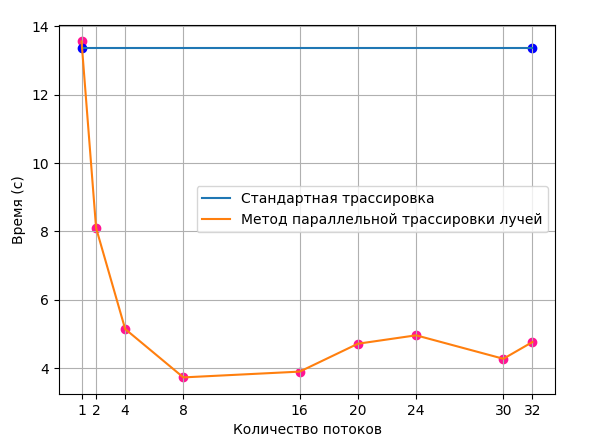
\includegraphics[width=0.7\textwidth]{time.png}
		\caption{Временные характеристики}
		\label{ref:time}}
\end{figure}

\newpage

Обычная реализация работает быстрее, чем создание одного потока,
потому что на создание потока тратится некоторое время.
При двух потоках выигрыш получается почти в два раза, так как два потока
трассируют одновременно свою часть экрана.
При увеличении числа потоков отслеживается уменьшение времени трассировки.
При 8 потоках достигается пик, при котором все ядра процессора одновременно
выполняют трассировку экрана.
Далее при увеличении числа потоков производительность падает.
Это объясняется тем, что создается очередь потоков, которая замедляет
работу программы.

\section{Вывод}

В данном разделе было произведено сравнение алгоритма трассировки лучей
при простой реализации и многопоточной (рис. \ref{ref:time}).
Результат показал, что выгоднее всего использовать все ядра процессора.